\documentclass[tikz, border=2pt]{standalone}

\usepackage{amsmath,amssymb}
\usepackage{xcolor}

\definecolor{utnblue}{RGB}{0, 51, 102}

\begin{document}
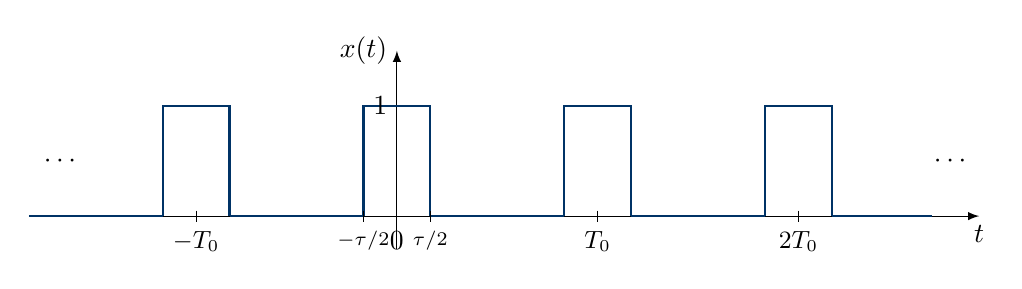
\begin{tikzpicture}[>=latex, xscale=0.85, yscale=1.4]
    % Eje
    \draw[->] (-5.5, 0) -- (8.7, 0) node[below] {$t$};
    \draw[->] (0, -0.3) -- (0, 1.5) node[left] {$x(t)$};

    % Pulsos: cada uno de ancho tau=1 centrado en k*T_0 con T_0=3
    % Pulso en t=-T_0=-3
    \draw[utnblue, thick] (-5.5, 0) -- (-3.5, 0);
    \draw[utnblue, thick] (-3.5, 0) -- (-3.5, 1) -- (-2.5, 1) -- (-2.5, 0);
    % Pulso en t=0
    \draw[utnblue, thick] (-2.5, 0) -- (-0.5, 0);
    \draw[utnblue, thick] (-0.5, 0) -- (-0.5, 1) -- (0.5, 1) -- (0.5, 0);
    % Pulso en t=T_0=3
    \draw[utnblue, thick] (0.5, 0) -- (2.5, 0);
    \draw[utnblue, thick] (2.5, 0) -- (2.5, 1) -- (3.5, 1) -- (3.5, 0);
    % Pulso en t=2T_0=6
    \draw[utnblue, thick] (3.5, 0) -- (5.5, 0);
    \draw[utnblue, thick] (5.5, 0) -- (5.5, 1) -- (6.5, 1) -- (6.5, 0);
    \draw[utnblue, thick] (6.5, 0) -- (8.0, 0);

    % Marcas y etiquetas
    \node[below] at (0, -0.05) {$0$};
    \draw (-3, 0.05) -- (-3, -0.05) node[below] {\small$-T_0$};
    \draw (3, 0.05) -- (3, -0.05) node[below] {\small$T_0$};
    \draw (6, 0.05) -- (6, -0.05) node[below] {\small$2T_0$};
    \draw (-0.5, 0.05) -- (-0.5, -0.05) node[below, font=\scriptsize] {$-\tau/2$};
    \draw (0.5, 0.05) -- (0.5, -0.05) node[below, font=\scriptsize] {$\tau/2$};
    \node[left] at (0, 1) {$1$};

    % Puntos suspensivos
    \node at (-5.0, 0.5) {$\cdots$};
    \node at (8.3, 0.5) {$\cdots$};
\end{tikzpicture}
\end{document}
